\chap{Enhanced Generative Adversarial Network}

\section{Introduction}
The original GAN as we discussed in the previous chapters, suffered from various key issues such as model collapse, difficulty in convergence which have resulted in poor quality image generation. Over the last couple of years the original GAN algorithm has been enhanced, tweaked and evolved by using latest advancement in deep neural networks. In this chapter, we discuss the architecture and methodologies which we have adopted in our work.  


\section{GAN Architecture} 

Before directly jumping to the condition GAN, lets look the baseline GAN which is the core system design of this work. Later in the next subsection, we will look at the changes which needed to be made for conditional image generation. 
\par
The original paper's\cite{Original-GAN} generator architecture consisted of rectifier linear\cite{RELU} and sigmoid activations, while the discriminator net used maxout [10] activations. The results were good but lacked stability and also suffered from the problem of model collapse.
\par
Later, Radford \textit{et al.}\cite{DCGAN} proposed deep convolution generative adversarial network. As the name suggests, they used deep convolution with fractional stride convolution and batch normalization to stabilize the model. This work uses DCGAN as the baseline architecture. The \cref{fig:DCGAN} shows the architecture of a generator and discriminator. In this work, we also use RELU as our activation function for all the layers expect in the output layer. As corroborated by the authors Radford \textit{et al.}\cite{DCGAN} RELU can help in convergence of the model and it also covers the color space of the distribution.
\par

By looking at the architecture of generator and discriminator, we notice that they are  opposite to each other. The generator uses up-convolution or commonly known as backward convolution to generate images. %J. Long, E. Shelhamer, and T. Darrell, “Fully convolutional networks for semantic segmentation,”CoRR, vol. abs/1411.4038, 2014. [Online]. Available: http://arxiv.org/abs/1411.4038
The discriminator is a standard deep convolution neural network used for classification of a real or a fake image.
\begin{figure}
  \centering
    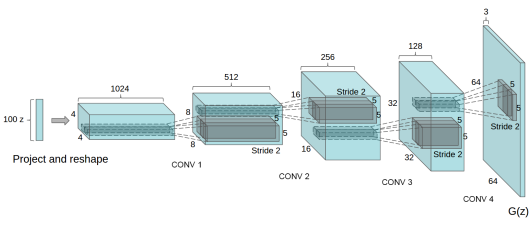
\includegraphics[scale=.7, angle=0]{Files/Generator-Architecture.png}
    \caption[Generator Architecture]{Generator Architecture\cite{DCGAN}}
    \label{fig:DCGAN}
\end{figure}

\subsection{Custom Architecture}

In this work we modify this architecture to generate  

\section{Training GAN}

Training a GAN is has always a tricky part and is still an ongoing research. This work uses DCGAN\cite{DCGAN} as baseline, as the DCGAN has shown that it can stabilize the networks to a great extent. The major contribution of the DCGAN in our work, is the use of Batch-Normalization, Strided Convolution and ADAM optimizer. We will go through each of these steps one by one.
\subsection{Batch Normalization}

Batch Normalization was first introduced by Ioffe  \textit{et al.}\cite{BatchNorm}. It is a major landmark in the area of deep learning as most of the current deep neural network frameworks contain batch normalization. 
To understand batch normalization, we need to understand the problem it is trying to solve. Its major aim is to minimize internal co-variance shift. Internal covariance shift refers to the change in input distribution as we are feeding data in mini batches. Since neural networks are designed in hierarchical fashion, even small change in the form of an outlier can get amplified, as we are dealing with generally more than a million parameters and several layers. To rectify this problem, we normalize each batch at every layer, by both mean and variance. This process is commonly called as whitning. The two major advantages of batch normalization are as follows.
\begin{itemize}
    \item Initial value of weights have less impact on gradient descent.
    \item It helps in keeping higher learning rate and accuracy. Hence it reduces overall training time and this helps in faster training of the GANs.
\end{itemize}

\subsection{Strided Convolution}

The concept of deconvolution was first introduced by Zeiler \textit{et al} \cite{Deconv}. It is also commonly known as  strided convolution, transposed fractional convolution or upsampling.

\par
It is basically going from output of some convolution to the input of that convolution. For instance, it is going from the green matrix which is a convolution kernel to the blue matrix as shown in the below figure. So given a kernel K, the type of convolution is defined by how forward or backward passes are calculated\cite{Deconv-Theano}.


\begin{figure}[H]
  \centering
    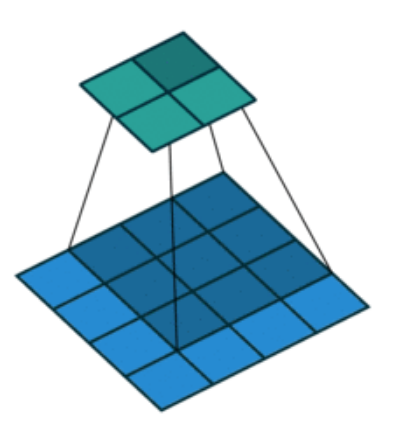
\includegraphics[scale=.5, angle=0]{Files/simple-conv.png}
    \caption[Simple Convolution]{Simple Convolution \cite{Deconv-Theano}}
    \label{fig: Simple Convolution}
  \centering
    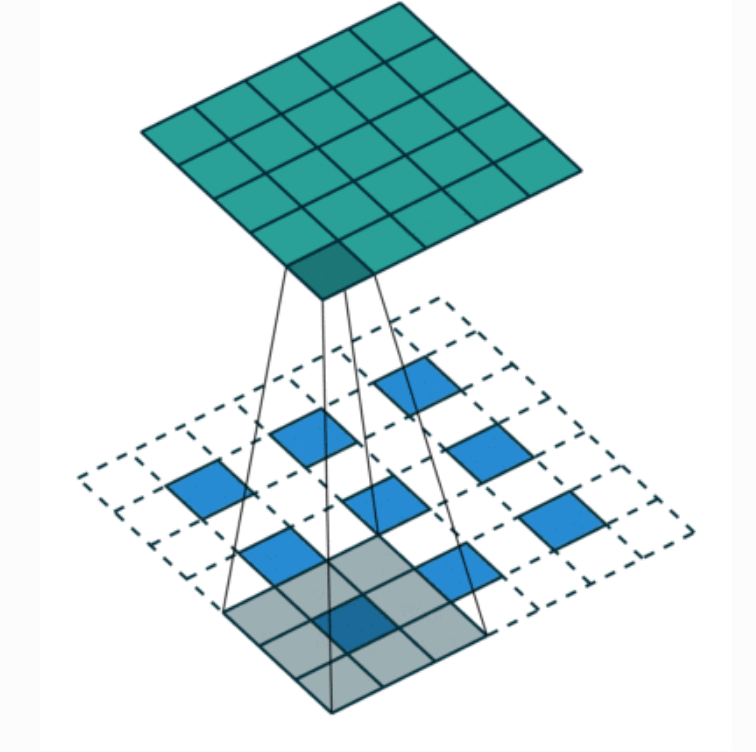
\includegraphics[scale=.4, angle=0]{Files/Frational-Stride-Conv.png}
    \caption[Transpose Convolution ]{Transpose Convolution \cite{Deconv-Theano}}
    \label{fig: Strided Convolution}
\end{figure}



\subsection{ADAM Optimizer}

Adaptive Moment Estimation, commonly known as ADAM optimizer is a stochastic gradient descent(SGD) optimizer. It was first proposed by Diederik \textit{et al.} \cite{Adam}. The vanilla stochastic gradient descent suffers from many problems. The three key issues which are directly related to our work are as follows:
\begin{itemize}
    \item In case of non convex error function, the neural network can be stuck at non local optima.
    \item Choosing correct learning is always a challenging task and it can cause longer time for SGD algorithm to converge.
    \item Specifically in our work, where we are trying to model the data and it is sparse, Vanilla SGD doesn't provide flexibility for having different learning rate for each weight.

To overcome these problems, we use ADAM optimizer in our work. It combines adagrade\cite{Adagrade} and momentum-optimizer \cite{momentum}. 

\end{itemize}
 
 
 